\begin{pages}
    \begin{Rightside}
    \selectlanguage{greek}
        \beginnumbering
        \pstart[
        			\chapter{Τὸ τοὺς δούλους σφραγίσαι}
        			\markboth{The Sealing of Servants}
				]
		Μετὰ τοῦτο εἶδον τέσσαρας ἀγγέλους ἑστῶτας ἐπὶ τὰς τέσσαρας γωνίας τῆς γῆς, κρατοῦντας τοὺς τέσσαρας ἀνέμους τῆς γῆς, ἵνα μὴ πνέῃ ἄνεμος ἐπὶ τῆς γῆς μήτε ἐπὶ τῆς θαλάσσης μήτε ἐπὶ πᾶν δένδρον. 
		\pend
		\pstart
		καὶ εἶδον ἄλλον ἄγγελον ἀναβαίνοντα ἀπὸ ἀνατολῆς ἡλίου, ἔχοντα σφραγῖδα Θεοῦ ζῶντος, καὶ ἔκραξεν φωνῇ μεγάλῃ τοῖς τέσσαρσιν ἀγγέλοις οἷς ἐδόθη αὐτοῖς ἀδικῆσαι τὴν γῆν καὶ τὴν θάλασσαν, λέγων Μὴ ἀδικήσητε τὴν γῆν μήτε τὴν θάλασσαν μήτε τὰ δένδρα, ἄχρι σφραγίσωμεν τοὺς δούλους τοῦ Θεοῦ ἡμῶν ἐπὶ τῶν μετώπων αὐτῶν. Καὶ ἤκουσα τὸν ἀριθμὸν τῶν ἐσφραγισμένων, ἑκατὸν τεσσεράκοντα τέσσαρες χιλιάδες ἐσφραγισμένοι ἐκ πάσης φυλῆς υἱῶν Ἰσραήλ·
		\pend 
		\pstart
		ἐκ φυλῆς Ἰούδα δώδεκα χιλιάδες ἐσφραγισμένοι, ἐκ φυλῆς Ῥουβὴν δώδεκα χιλιάδες, ἐκ φυλῆς Γὰδ δώδεκα χιλιάδες, ἐκ φυλῆς Ἀσὴρ δώδεκα χιλιάδες, ἐκ φυλῆς Νεφθαλεὶμ δώδεκα χιλιάδες, ἐκ φυλῆς Μανασσῆ δώδεκα χιλιάδες, ἐκ φυλῆς Συμεὼν δώδεκα χιλιάδες, ἐκ φυλῆς Λευεὶ δώδεκα χιλιάδες, ἐκ φυλῆς Ἰσσαχὰρ δώδεκα χιλιάδες, ἐκ φυλῆς Ζαβουλὼν δώδεκα χιλιάδες, ἐκ φυλῆς Ἰωσὴφ δώδεκα χιλιάδες, ἐκ φυλῆς Βενιαμεὶν δώδεκα χιλιάδες ἐσφραγισμένοι.
		\pend
		\pstart
		Μετὰ ταῦτα εἶδον, καὶ ἰδοὺ ὄχλος πολύς, ὃν ἀριθμῆσαι αὐτὸν οὐδεὶς ἐδύνατο, ἐκ παντὸς ἔθνους καὶ φυλῶν καὶ λαῶν καὶ γλωσσῶν, ἑστῶτες ἐνώπιον τοῦ θρόνου καὶ ἐνώπιον τοῦ Ἀρνίου, περιβεβλημένους στολὰς λευκάς, καὶ φοίνικες ἐν ταῖς χερσὶν αὐτῶν· καὶ κράζουσιν φωνῇ μεγάλῃ λέγοντες Ἡ σωτηρία τῷ Θεῷ ἡμῶν τῷ καθημένῳ ἐπὶ τῷ θρόνῳ καὶ τῷ Ἀρνίῳ.
		\pend
		\pstart
		καὶ πάντες οἱ ἄγγελοι εἱστήκεισαν κύκλῳ τοῦ θρόνου καὶ τῶν πρεσβυτέρων καὶ τῶν τεσσάρων ζῴων, καὶ ἔπεσαν ἐνώπιον τοῦ θρόνου ἐπὶ τὰ πρόσωπα αὐτῶν καὶ προσεκύνησαν τῷ Θεῷ, λέγοντες Ἀμήν, ἡ εὐλογία καὶ ἡ δόξα καὶ ἡ σοφία καὶ ἡ εὐχαριστία καὶ ἡ τιμὴ καὶ ἡ δύναμις καὶ ἡ 	ἰσχὺς τῷ Θεῷ ἡμῶν εἰς τοὺς αἰῶνας τῶν αἰώνων· ἀμήν.
		\pend
		\pstart
		Καὶ ἀπεκρίθη εἷς ἐκ τῶν πρεσβυτέρων λέγων μοι Οὗτοι οἱ περιβεβλημένοι τὰς στολὰς τὰς λευκὰς τίνες εἰσὶν καὶ πόθεν ἦλθον; καὶ εἴρηκα αὐτῷ Κύριέ μου, σὺ οἶδας. καὶ εἶπέν μοι Οὗτοί εἰσιν οἱ ἐρχόμενοι ἐκ τῆς θλίψεως τῆς μεγάλης, καὶ ἔπλυναν τὰς στολὰς αὐτῶν καὶ ἐλεύκαναν αὐτὰς ἐν τῷ αἵματι τοῦ Ἀρνίου. διὰ τοῦτό εἰσιν ἐνώπιον τοῦ θρόνου τοῦ Θεοῦ, καὶ λατρεύουσιν αὐτῷ ἡμέρας καὶ νυκτὸς ἐν τῷ ναῷ αὐτοῦ, καὶ ὁ καθήμενος ἐπὶ τοῦ θρόνου σκηνώσει ἐπ’ αὐτούς. οὐ πεινάσουσιν ἔτι οὐδὲ διψήσουσιν ἔτι, οὐδὲ μὴ πέσῃ ἐπ’ αὐτοὺς ὁ ἥλιος οὐδὲ πᾶν καῦμα, ὅτι τὸ Ἀρνίον τὸ ἀνὰ μέσον τοῦ θρόνου ποιμανεῖ αὐτούς καὶ ὁδηγήσει αὐτοὺς ἐπὶ ζωῆς πηγὰς ὑδάτων· καὶ ἐξαλείψει ὁ Θεὸς πᾶν δάκρυον ἐκ τῶν ὀφθαλμῶν αὐτῶν.
		\pend
        \endnumbering
    \end{Rightside}
    \begin{Leftside}
        \beginnumbering
        \pstart[
        			\chapter{The Sealing of Servants}
				]
		After this I saw four angels standing upon the four corners of the Earth (and I saw them) taking the seven winds of the Earth, so that (the) wind shall not blow on the (face of the) Earth nor on (over?) the sea, nor on all (any) trees.
		\pend
		\pstart
		And I saw another angel coming down from the East (lit. Eastern sun), having (in his hands) the seal of the living God; and he was shouting in a great voice to the four angels — (those) to whom (the authority) to hurt the Earth and the sea was given — saying, “Do not harm the Earth, nor the sea, nor the trees until we seal the servants of our God upon their foreheads. And I heard the number of the sealed (and that number was) one-hundred forty-four thousand (sealed) from every tribe of the children of Israel:
		\pend
		\pstart
		From the tribe of Juda (there were) twelve-thousand sealed; from the tribe of Ruben twelve-thousand; from the tribe of Gad twelve-thousand; from the tribe of Aser twelve-thousand; from the tribe of Naphthalim twelve-thousand; from the tribe of Manasses twelve-thousand; from the tribe of Simeon twelve-thousand; from the tribe of Levi twelve-thousand; from the tribe of Issachar twelve-thousand; from the tribe of Zabulon twelve-thousand; from the tribe of Joseph twelve-thousand; (and) from the tribe of Benjamin (there were) twelve-thousand sealed.
		\pend
		\pstart
		After this I saw — and look! — a great crowd (the number of people in) which nobody was able to count, from every people and tribe and nation and tongue (language); (and they were) standing before the throne and before the Lamb (and they were all) clad in long, white robes and (they all had) palms (date palms, type of tree) in their hands. And they shout(ed) in a great voice saying, “(The) salvation (be) to our God and to the One sitting upon the throne and to the Lamb.”
		\pend
		\pstart
		And all the angels and elders and the four creatures were standing around the throne and they fell to their face before the throne and worshipped God saying, “Amen. The blessing and glory and wisdom and gratitude and power and might and strength (be) to our God into the eternity of eternities. Amen.”
		\pend
		\pstart
		And of the elders (there was one) answering and telling me, “Those (over there), the ones who are clad in the white robes — who are they and where did they come from?” And I told him, “My lord, you know.” And he said to me, “They are those who come from the great oppression and they washed their robes and whitened them in (with) the blood of the Lamb. Because of (through) this, they are before the throne of God and they serve Him in His temple day and night; and He who sits upon the throne will erect his tent (dwell, live) on them. And they are neither hungry nor thirsty anymore; nor will the Sun fall upon them (shine on them?) nor all (any) heat. For the Lamb which is in the middle of the throne will feed them and show them the way to the living fountain of waters; and God will wipe away every tear from their eyes. 
		\pend
        \endnumbering
    \end{Leftside}

\end{pages} 
\Pages

\clearpage
\thispagestyle{empty}
\null\vfill
\settowidth\longest{\huge\itshape […] and when I turned around I saw}
\begin{center}
\parbox{\longest}{%
  \raggedright{\huge\itshape%
    ``After this I saw four angels standing upon the four corners of the Earth (and I saw them) taking the seven winds of the Earth […]'' \par\bigskip
  }
  \raggedleft\Large\MakeUppercase{``Apocalypse flamande'' — \nth{15} century}\par%
}
\vfill\vfill
\clearpage\newpage
\end{center}
\newpage
\thispagestyle{empty}
\begin{center}
	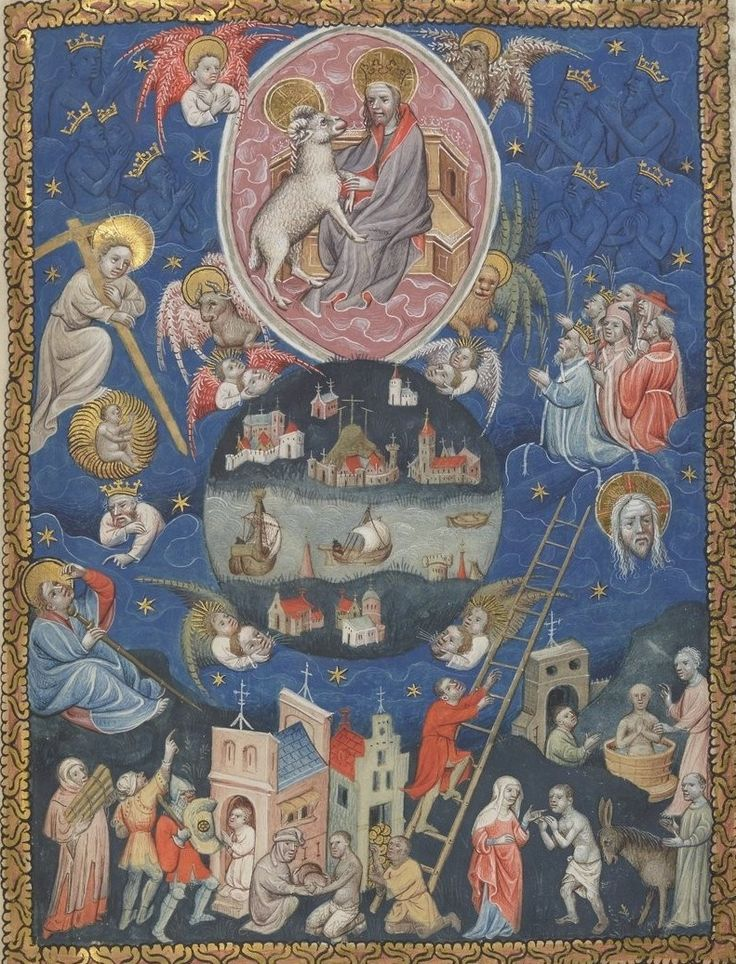
\includegraphics[width=1\textwidth]{images/illustrations/angelsholdingwinds.jpg}
\end{center}